\documentclass[11pt]{article}

\usepackage[margin=1in]{geometry}
\usepackage[T1]{fontenc}
\usepackage{lmodern}
\usepackage{microtype}
\usepackage{amsmath,amssymb,amsthm,mathtools}
\usepackage{mathrsfs}
\usepackage[dvipsnames]{xcolor}
\usepackage[most]{tcolorbox}
\usepackage{tikz}
\usetikzlibrary{decorations.markings,patterns}
\usepackage{enumitem}
\usepackage{tocloft}
\usepackage[hidelinks]{hyperref}

\definecolor{courseblue}{HTML}{1F4E79}
\definecolor{lightblue}{HTML}{EAF2F8}
\definecolor{lightgreen}{HTML}{EAF7EA}
\definecolor{lightpink}{HTML}{FCE8EF}
\definecolor{lightyellow}{HTML}{FFF8D6}
\definecolor{warningyellow}{HTML}{D6A000}
\definecolor{exercisebg}{HTML}{FDEAEA}
\definecolor{exerciseframe}{HTML}{B54040}
\definecolor{examplebg}{HTML}{F4FAFE}
\definecolor{exampleframe}{HTML}{85C1E9}
\definecolor{darkgray}{HTML}{333333}
\definecolor{lightorange}{HTML}{FDEBD8}
\definecolor{orangeframe}{HTML}{E08A3C}
\definecolor{remarkbg}{HTML}{F3EEFB}
\definecolor{remarkframe}{HTML}{9B7FC9}

\setlength{\parindent}{0pt}
\setlength{\parskip}{0.45em}
\setlist[itemize]{topsep=0.25em,itemsep=0.15em}
\renewcommand{\cftsecleader}{\cftdotfill{\cftdotsep}}
\renewcommand{\cftsubsecleader}{\cftdotfill{\cftdotsep}}

\theoremstyle{plain}
\newtheorem{theorem}{Theorem}[section]
\newtheorem{proposition}[theorem]{Proposition}
\newtheorem{lemma}[theorem]{Lemma}
\newtheorem{corollary}[theorem]{Corollary}
\theoremstyle{definition}
\newtheorem{definition}[theorem]{Definition}
\newtheorem{example}[theorem]{Example}
\newtheorem{exercise}[theorem]{Exercise}
\theoremstyle{remark}
\newtheorem*{remark}{Remark}
\newtheorem*{fact}{Fact}
\newtheorem*{warning}{Warning}

\tcolorboxenvironment{definition}{
  enhanced,
  unbreakable,
  colback=lightgreen,
  colframe=ForestGreen,
  boxrule=0.7pt,
  arc=2pt,
  left=6pt,
  right=6pt,
  top=5pt,
  bottom=5pt
}

\tcolorboxenvironment{remark}{
  enhanced,
  colback=remarkbg,
  colframe=remarkframe,
  before upper={\setlength{\parskip}{0.5em}},
  boxrule=0.7pt,
  arc=2pt,
  left=6pt,
  right=6pt,
  top=5pt,
  bottom=5pt
}

\tcolorboxenvironment{warning}{
  enhanced,
  colback=lightyellow,
  colframe=warningyellow,
  boxrule=0.7pt,
  arc=2pt,
  left=6pt,
  right=6pt,
  top=5pt,
  bottom=5pt
}

\tcolorboxenvironment{exercise}{
  enhanced,
  colback=exercisebg,
  colframe=exerciseframe,
  boxrule=1pt,
  arc=2pt,
  left=6pt,
  right=6pt,
  top=5pt,
  bottom=5pt
}

\tcolorboxenvironment{example}{
  enhanced,
  colback=examplebg,
  colframe=exampleframe,
  boxrule=0.7pt,
  arc=2pt,
  left=6pt,
  right=6pt,
  top=5pt,
  bottom=5pt
}

\numberwithin{equation}{section}

\newcommand{\be}{\begin{eqnarray}}
\newcommand{\ee}{\end{eqnarray}}
\newcommand{\C}{\mathbb{C}}
\newcommand{\R}{\mathbb{R}}
\newcommand{\N}{\mathbb{N}}
\newcommand{\Z}{\mathbb{Z}}
\DeclareMathOperator{\Log}{Log}
\DeclareMathOperator{\Arg}{Arg}

\DeclareMathOperator{\Hol}{\mathcal{H}\mathrm{ol}}
\DeclareMathOperator{\Real}{Re}
\DeclareMathOperator{\Imag}{Im}
\newcommand{\A}{\mathcal{A}}
\newcommand{\CT}{\C[[T]]}
\newcommand{\CLT}{\C((T))}
\tcbset{breakable}
% Compact spacing around diagrams; keep the main text at 11pt.
\newenvironment{lecturefigure}
 {\par\addvspace{0.25em}\begingroup\setlength{\parskip}{0pt}\centering}
 {\par\endgroup\addvspace{0.25em}}
\begin{document}

\begin{center}
  \colorbox{lightblue}{%
    \begin{minipage}{0.94\textwidth}
      \vspace{0.55em}
      \begin{tabular*}{\textwidth}{@{\extracolsep{\fill}}lr}
        {\color{courseblue}\bfseries\LARGE Lecture 25} &
        {\color{courseblue}\bfseries\LARGE MATH 411}\\[0.35em]
        \textbf{Fall 2026} & \textbf{Date: Nov 16, 2026}\\
        & \textbf{Instructor: Manish Patnaik}
      \end{tabular*}
      \vspace{0.45em}
    \end{minipage}}
\end{center}

\setcounter{tocdepth}{1}
\tableofcontents
\vspace{0.45em}

% Sources: handwritten Lecture 23, pages 7--8 (improper integrals), and
% handwritten Lecture 24, pages 1--3 (meromorphic functions, orders,
% and the argument principle).
% Added: a lemma on zeros of holomorphic functions.
In Lecture~24 we used the residue theorem to compute trigonometric
integrals. Today we use it to evaluate improper integrals over the real
line, then study the order of zeros and poles and prove the argument
principle.

\section{Recall: the residue theorem}
Let $f$ be holomorphic on an open set $U$ except at isolated singularities
$z_1,\dots,z_n$. If $\gamma$ is a closed piecewise $C^1$ curve in
$U\setminus\{z_1,\dots,z_n\}$ that is null-homotopic in $U$, then
\[
 \int_\gamma f(z)\,dz=2\pi i\sum_{j=1}^{n}
 w(\gamma,z_j)\,\operatorname{Res}_{z_j}(f).
\]
Here $w(\gamma,z_j)$ is the winding number and $\operatorname{Res}_{z_j}(f)$
is the coefficient of $(z-z_j)^{-1}$ in the Laurent expansion. For a simple
closed counterclockwise contour, the sum includes exactly the singularities
inside the contour, each with winding number $1$.


Recall also from Lecture~24
that if $p$ and $q$ are holomorphic near $z_0$ and $q$ has a simple zero
there,  $$\operatorname{Res}_{z_0}(p/q)=p(z_0)/q'(z_0).$$

\section{Improper integrals over the real line}
% Handwritten Lecture 23, pages 7--8. The handwritten notes split
% [-R,R] into [-R,0] and [0,R]; here they are combined. The example on
% page 8 is completed here.
We now compute improper integrals of the form
$\int_{-\infty}^{\infty}f(x)\,dx$. Recall that by definition, this integral is equal to the limit
\[
 \int_{-\infty}^{\infty}f(x)\,dx=\lim_{R\to\infty}\int_{-R}^{R}f(x)\,dx,
\] assuming the right hand side exists.
Assume now that $f(x)$ is the restriction to $\R$ of a function $f(z)$ that is
holomorphic on a half-plane $\{\Imag z>-\epsilon\}$ except for finitely
many poles, none of which lie on the real axis. (This holds, for
example, for a rational function with no real poles.)

Let $H=\{z:\Imag z>0\}$ be the upper half-plane. For $R>0$ let $\gamma_R$
be the closed curve consisting of the segment $[-R,R]$ followed by the
semicircle $C_R(t)=Re^{it}$, $0\leq t\leq\pi$.

\begin{lecturefigure}
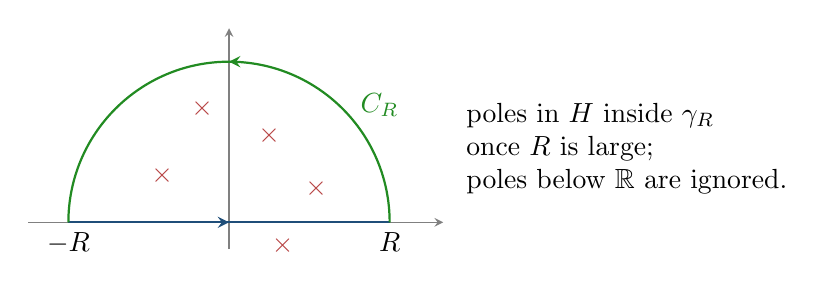
\begin{tikzpicture}[scale=0.85,>=stealth]
 \draw[gray,->] (-3,0)--(3.2,0);
 \draw[gray,->] (0,-0.4)--(0,2.9);
 \draw[courseblue,thick,postaction={decorate},decoration={markings,
  mark=at position 0.5 with {\arrow{>}}}] (-2.4,0)--(2.4,0);
 \draw[ForestGreen,thick,postaction={decorate},decoration={markings,
  mark=at position 0.5 with {\arrow{>}}}] (2.4,0) arc(0:180:2.4);
 \foreach \p in {(-1,0.7),(0.6,1.3),(1.3,0.5),(-0.4,1.7)}
  \node[exerciseframe] at \p {$\times$};
 \node[exerciseframe] at (0.8,-0.35) {$\times$};
 \node[below] at (-2.4,0) {$-R$};
 \node[below] at (2.4,0) {$R$};
 \node[ForestGreen] at (2.25,1.75) {$C_R$};
 \node[right,align=left] at (3.4,1.1)
 {poles in $H$ inside $\gamma_R$\\ once $R$ is large;\\ poles below $\R$ are ignored.};
\end{tikzpicture}
\end{lecturefigure}

The half-plane $\{\Imag z>-\epsilon\}$ is convex, hence simply connected.
Once $R$ exceeds the moduli of all poles $z_j$ in $H$, each such pole has
$w(\gamma_R,z_j)=1$, while any pole below the real axis lies outside
$\gamma_R$ and has winding number $0$. The residue theorem gives
\[
 \int_{-R}^{R}f(x)\,dx+\int_{C_R}f(z)\,dz
 =\int_{\gamma_R}f
 =2\pi i\sum_{z_j\in H}\operatorname{Res}_{z_j}(f).
\]


\begin{theorem}\label{thm:improper}
Let $f$ be as above, and suppose there are $B>0$ and $R_0>0$ with
\[
 |f(z)|\leq\frac{B}{|z|^2}\qquad(\Imag z\geq0,\ |z|\geq R_0).
\]
Then
\[
 \boxed{\displaystyle\int_{-\infty}^{\infty}f(x)\,dx
 =2\pi i\sum_{z_j\in H}\operatorname{Res}_{z_j}(f),}
\]
the sum being over the poles of $f$ in the upper half-plane.
\end{theorem}
\begin{proof}
The bound gives absolute convergence on the real line. Thus the improper
integral equals $\lim_{R\to\infty}\int_{-R}^Rf$. For $R\geq R_0$, the
ML estimate gives
\[
 \left|\int_{C_R}f\right|
 \leq\operatorname{ArcLength}(C_R)\,\|f\|_{C_R}
 \leq\pi R\cdot\frac{B}{R^2}=\frac{\pi B}{R}\longrightarrow0.
\]
Letting $R\to\infty$ in the identity above gives the result.
\end{proof}

\begin{remark}
The same argument works if $|f(z)|\leq B/|z|^{1+a}$ for some $a>0$: the
semicircle integral is then at most $\pi B/R^a$.
\end{remark}

\begin{example}
We compute $\displaystyle\int_{-\infty}^{\infty}\frac{dx}{x^4+1}$, using
$f(z)=1/(z^4+1)$. For $|z|\geq2$ we have $|z^4+1|\geq|z|^4-1\geq|z|^4/2$,
so $|f(z)|\leq2/|z|^4\leq1/(2|z|^2)$ and Theorem~\ref{thm:improper} applies.
The poles are the fourth roots of $-1$, namely $e^{i\pi/4}$,
$e^{3i\pi/4}$, $e^{5i\pi/4}$, $e^{7i\pi/4}$; the first two lie in $H$.
At each pole $z_0$, the simple-pole formula from the review gives
\[
 \operatorname{Res}_{z_0}f=\frac{1}{4z_0^3}=\frac{z_0}{4z_0^4}=-\frac{z_0}{4}.
\]
Since $e^{i\pi/4}+e^{3i\pi/4}=i\sqrt2$,
\[
 \boxed{\int_{-\infty}^{\infty}\frac{dx}{x^4+1}
 =2\pi i\cdot\Bigl(-\frac{i\sqrt2}{4}\Bigr)=\frac{\pi}{\sqrt2}.}
\]
\end{example}

%\begin{exercise}
%Use Theorem~\ref{thm:improper} to show that
%$\displaystyle\int_{-\infty}^{\infty}\frac{dx}{(x^2+1)^2}=\frac{\pi}{2}$.
%\end{exercise}

\section{Meromorphic functions and the order of a zero or pole}
% Handwritten Lecture 24, pages 1--2.
A function $f$ is \emph{meromorphic} on an open set $U$ if it is
holomorphic on $U$ except for poles, in other words it has isoalted singularities in $U$ except which are either removable or poles, i.e. no essential singularities.

\subsection{Zeros of holomorphic functions}
We recall a fact here about zero; it follows from results we proved for analytic functions in Lecture~10 (so I will skip the proof in class, but here it is for completeness.)

\begin{lemma}[Zeros are isolated]\label{lem:zeros}
Let $D$ be a connected open set and $F$ holomorphic on $D$, not
identically zero. Then:
\begin{enumerate}
 \item at each zero $z_0$ of $F$ there are an integer $m\geq1$ and a
 function $g$ holomorphic near $z_0$ with $g(z_0)\ne0$ such that
 $F(z)=(z-z_0)^mg(z)$; in particular $z_0$ is an isolated zero;
 \item $F$ has only finitely many zeros in each compact subset of $D$.
\end{enumerate}
\end{lemma}
\begin{proof}
Let $S=\{z\in D:\ F^{(k)}(z)=0\text{ for all }k\geq0\}$. Each derivative
is continuous, so $S$ is closed in $D$. If $z\in S$, the Taylor series of
$F$ at $z$ is zero, and it represents $F$ on a disc around $z$
(Lecture~20); so $F\equiv0$ on that disc, which therefore lies in $S$.
Thus $S$ is also open. Since $D$ is connected and $S\ne D$, we get
$S=\emptyset$.

(1) At a zero $z_0$, let $m\geq1$ be the least $k$ with
$F^{(k)}(z_0)\ne0$. The Taylor series at $z_0$ starts with
$a_m(z-z_0)^m$, $a_m\ne0$, so $F=(z-z_0)^mg$ with
$g(z)=a_m+a_{m+1}(z-z_0)+\cdots$. Since $g(z_0)\ne0$ and $g$ is
continuous, $g$ and hence $F$ has no other zeros near $z_0$.

(2) If $K\subseteq D$ is compact and contains infinitely many zeros, they
accumulate at some $p\in K$. By continuity $F(p)=0$, and $p$ is not an
isolated zero, contradicting (1).
\end{proof}

\subsection{Order and the logarithmic derivative}
Let $f$ be meromorphic near $z_0$ and not identically zero near $z_0$. By
Lemma~\ref{lem:zeros} if $f(z_0)=0$, and by the Laurent expansion
(Lecture~22) if $z_0$ is a pole, we can write
\[
 f(z)=(z-z_0)^m\,g(z),\qquad g\text{ holomorphic near }z_0,\quad g(z_0)\ne0,
\]
for a unique integer $m$. Equivalently, $f(z)=a_m(z-z_0)^m(1+h(z))$ with
$a_m=g(z_0)\ne0$ and $h$ holomorphic, $h(z_0)=0$.

\begin{definition}
The integer $m=\operatorname{ord}_{z_0}(f)$ is the \emph{order} of $f$
at $z_0$. If $m>0$, $f$ has a \emph{zero of order $m$}; if $m<0$, $f$ has a
\emph{pole of order $-m$}. For example, $m=-1$ means
$f=\frac{a_{-1}}{z-z_0}+\cdots$, a pole of order $1$.
\end{definition}

By the product rule $(fg)'=f'g+fg'$, so
\[
 \frac{(fg)'}{fg}=\frac{f'}{f}+\frac{g'}{g}.
\]
The quotient $f'/f$ is called the \emph{logarithmic derivative} of $f$,
written $d\log(f)$, since formally $(\log f)'=f'/f$. The identity says
$d\log(fg)=d\log(f)+d\log(g)$. Applying it to $f=(z-z_0)^m\cdot g$,
\[
 \frac{f'}{f}=\frac{m}{z-z_0}+\frac{g'}{g}.
\]
Since $g(z_0)\ne0$, $g'/g$ is holomorphic near $z_0$. Hence
\[
 \boxed{\operatorname{Res}_{z_0}\Bigl(\frac{f'}{f}\Bigr)
 =m=\operatorname{ord}_{z_0}(f).}
\]

\section{The argument principle}
% Handwritten Lecture 24, pages 2--3.
Combining this observation with the residue theorem:

\begin{theorem}\label{thm:log-derivative}
Let $U$ be open and $f$ meromorphic on $U$ with finitely many zeros and
poles $z_1,\dots,z_n$. Let $\gamma$ be a closed piecewise $C^1$ curve in
$U\setminus\{z_1,\dots,z_n\}$ that is null-homotopic in $U$. Then
\[
 \int_\gamma\frac{f'}{f}=2\pi i\sum_{j=1}^{n}w(\gamma,z_j)\,
 \operatorname{ord}_{z_j}(f).
\]
\end{theorem}
\begin{proof}
On $U\setminus\{z_1,\dots,z_n\}$, $f$ is holomorphic and nonvanishing, so
$f'/f$ is holomorphic there. At each $z_j$ it has residue
$\operatorname{ord}_{z_j}(f)$ by the computation above. Apply the residue
theorem to $f'/f$.
\end{proof}

\begin{example}
Let $f(z)=\dfrac{(z-1)^2}{(z+2)^3}$, with a zero of order $2$ at $1$ and a
pole of order $3$ at $-2$. For the circle $|z|=3$, both points are inside
and $\int f'/f=2\pi i(2-3)=-2\pi i$. For $|z|=\tfrac32$, only $1$ is inside
and $\int f'/f=4\pi i$. Directly,
$f'/f=\frac{2}{z-1}-\frac{3}{z+2}$.
\end{example}

\newpage
Choosing $\gamma$ to be a circle gives the following.

\begin{corollary}[Argument principle]\label{cor:argument}
Let $C$ be a positively oriented circle bounding the open disc $D$, and
let $f$ be meromorphic on an open set $W\supseteq\overline D$, with finitely
many zeros and poles in $W$, none on $C$. Then
\[
 \boxed{\frac{1}{2\pi i}\int_C\frac{f'}{f}
 =\#\{\text{zeros of $f$ in $D$}\}-\#\{\text{poles of $f$ in $D$}\},}
\]
where zeros and poles are counted with multiplicity (that is, with their
orders).
\end{corollary}
\begin{proof}
Let $D=D(c,r)$. By compactness of $\overline D$ there is $\rho>r$ with
$D(c,\rho)\subseteq W$. Apply Theorem~\ref{thm:log-derivative} on the
convex, hence simply connected, set $U=D(c,\rho)$. It remains to note that
$w(C,\alpha)=1$ for $\alpha\in D$ (Cauchy's formula with $f=1$) and
$w(C,\alpha)=0$ for $|\alpha-c|>r$ (since $1/(z-\alpha)$ is holomorphic on
the disc $D(c,|\alpha-c|)$, which contains $C$).
\end{proof}

\begin{lecturefigure}
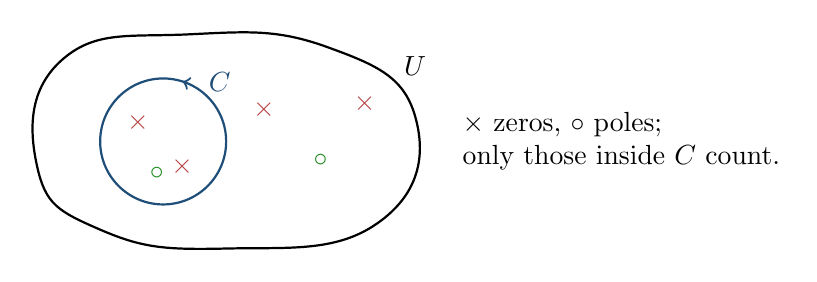
\begin{tikzpicture}[scale=0.8]
 \draw[thick] plot[smooth cycle,tension=0.8] coordinates
 {(-3,-0.4) (-2.6,1.3) (-0.6,1.7) (1.6,1.5) (3,0.4)
  (2.4,-1.3) (0,-1.7) (-2,-1.4)};
 \node at (3,1.2) {$U$};
 \draw[courseblue,thick,postaction={decorate},decoration={markings,
  mark=at position 0.2 with {\arrow{>}}}] (-1,0) circle(1);
 \node[courseblue] at (-0.1,0.95) {$C$};
 \node[exerciseframe] at (-1.4,0.3) {$\times$};
 \node[exerciseframe] at (-0.7,-0.4) {$\times$};
 \node[ForestGreen] at (-1.1,-0.5) {$\circ$};
 \node[exerciseframe] at (0.6,0.5) {$\times$};
 \node[ForestGreen] at (1.5,-0.3) {$\circ$};
 \node[exerciseframe] at (2.2,0.6) {$\times$};
 \node[right,align=left] at (3.6,0)
 {$\times$ zeros, $\circ$ poles;\\ only those inside $C$ count.};
\end{tikzpicture}
\end{lecturefigure}

\begin{remark}[Why ``argument'']
If $C$ is parametrized by $\gamma(t)$, $0\leq t\leq2\pi$, then
$\int_C f'/f=\int_0^{2\pi}\frac{(f\circ\gamma)'(t)}{f(\gamma(t))}\,dt
=\int_{f\circ C}\frac{dw}{w}$. So the left side of the argument principle
is $w(f\circ C,0)$: the number of times the image curve $f\circ C$ winds
around $0$, i.e.\ the total change in $\arg f(z)$ around $C$, divided by
$2\pi$.
\end{remark}

\end{document}
